\chapter{Experiments and validation}
\label{chap:validation}

This chapter contains...
\todo[inline]{Add diagram of testing process}

\section{PID controller validation}
\label{sec:test-1-pid}

% Process of tuning the PIDs
% Graphs from test-controller
% Analysis of error

\todo[inline]{Flow chart of validation process}
\todo[inline]{Videos for github}

As has been mentioned before, the velocity controller that is the heart of the person following mechanism is based on two PID controllers.
In order to get velocity outputs for the PID controllers that produce a stable movement of the vehicle, it is necessary to tune the parameters of the controllers until the appropriate combination is found.
The value for the coefficients used for the project has been found empirically with the help of the tuning tool described in section~\ref{subsec:test-tools} and developed for this purpose, and its performance validated with the controller testing tool, both running in a simulated environment with the flight stack in SITL mode so that it is possible to take continuous measures of the response of the PID controllers to step movements of a simulated person present in the 3D world.
In the first place, each of the controllers has been tuned independently of the other by allowing the vehicle only one direction of movement at a time.
Afterwards, both controllers are engaged at the same time to take measurements of their joint response to a range of different inputs.

The controllers are calibrated for a starting position of x=0, y=0 for the vehicle and x=600, y=0 for the person in world coordinates of the simulated environment.
At these position, the processing of the images taken from the simulated camera detects the person centered in the field of view and with a height of 36\% of the image height.
The set points for the controllers running in the simulator are therefore 0.5 for the yaw controller and 0.36 for the forward controller.

\subsection{Yaw controller}

\begin{figure}
  \centering
  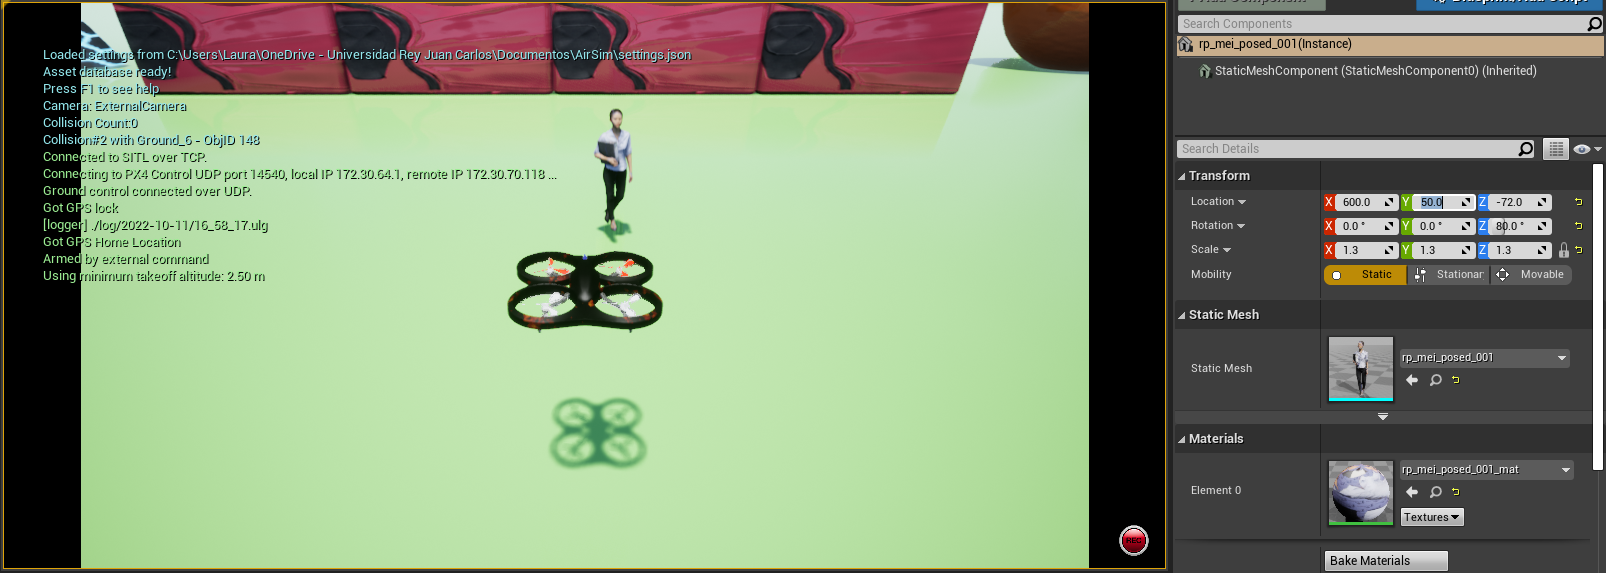
\includegraphics[width=\textwidth, keepaspectratio]{img/4.1-tune/sim_window_tune.png}
  \caption{Starting position of the simulator for tuning the yaw controller}\label{fig:sim_window_tune}
\end{figure}

\begin{figure}
  \centering
  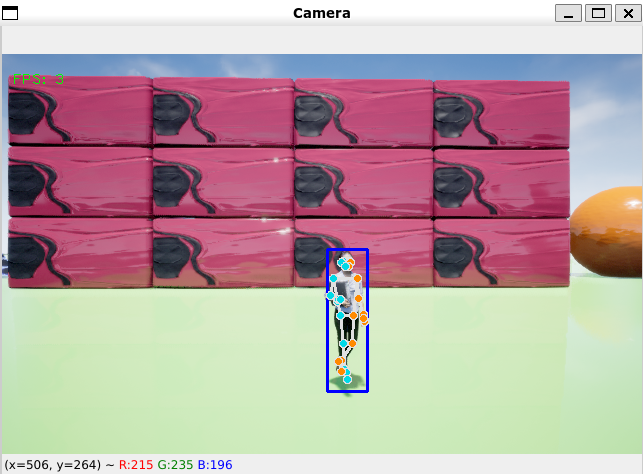
\includegraphics[width=.5\textwidth, keepaspectratio]{img/4.1-tune/yaw_tune_start_pos.png}
  \caption{Perspective from the vehicle at the start of the program run}\label{fig:sim_camera_tune}
\end{figure}

To find the correct coefficients for the controller that governs the yaw velocity of the vehicle, the target person is set in a position slightly to the side on its field of view so that when the controller is engaged it produces a rotation of the vehicle to that side.
Figure~\ref{fig:sim_window_tune} shows the starting position of the simulated environment before each run, where the 3D model has been situated at (600,50), that is, 50 units to the right of the target position.
The image captured from the simulated camera is shown in figure~\ref{fig:sim_camera_tune}.

\begin{figure}
  \centering
  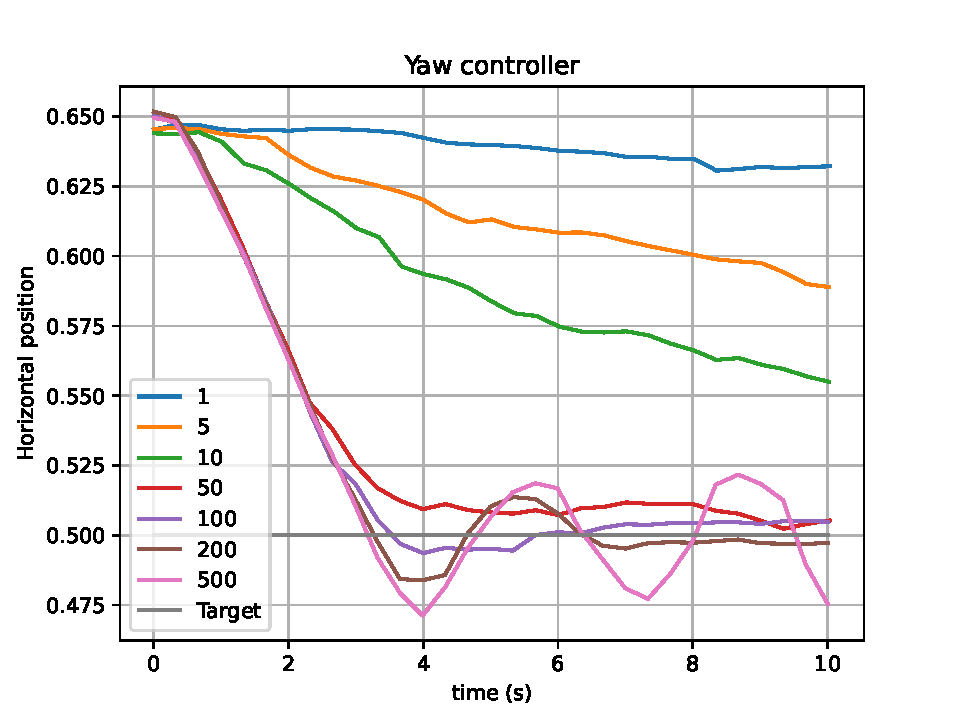
\includegraphics[width=.45\linewidth]{img/4.1-tune/yaw_p1_feedback.pdf}
  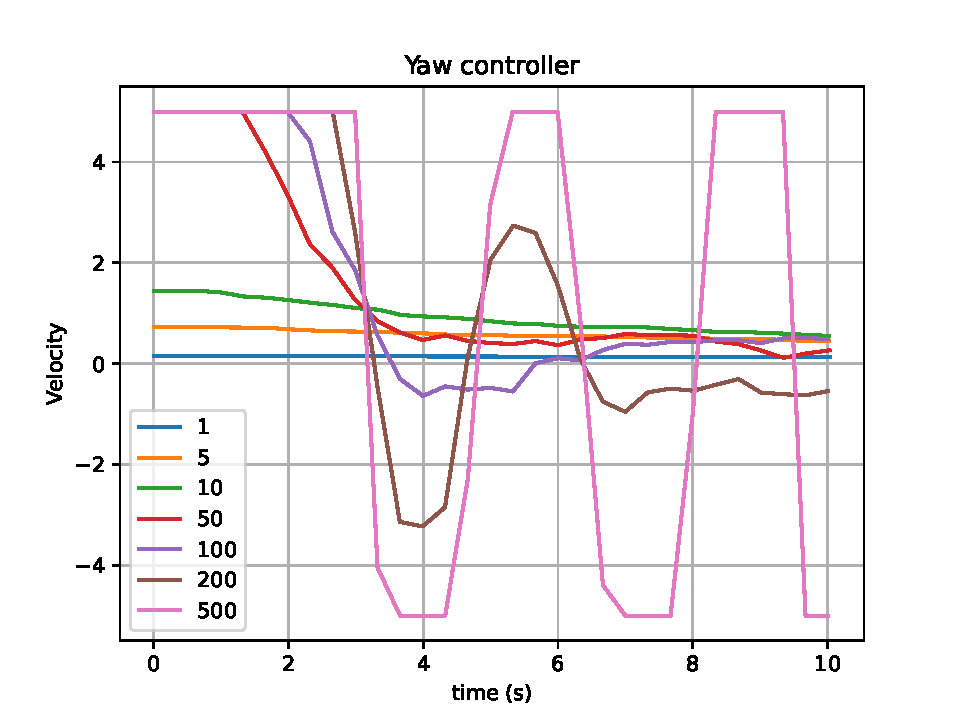
\includegraphics[width=.45\linewidth]{img/4.1-tune/yaw_p1_speed.pdf}
  \caption{Variation of (a) input position and (b) output velocity for different values of $K_{P}$ while the yaw controller is engaged.}\label{fig:tune-yaw-prop}
\end{figure}


The first step taken is to test different values of $K_{P}$ while maintaining $K_{I}$ and $K_{D}$ at zero.
Figure~\ref{fig:tune-yaw-prop} shows the output of the tuning program for the tested values of $K_{P}$.
The left graph represents the variation of the horizontal position detected by the camera for the first 10 seconds after activating the controller and the right graph, the velocity that the controller outputs to the pilot module to reach the target.
It can be seen that for low values of $K_{P}$, the controller makes the vehicle move too slowly towards its target, so that it takes more than the 10 seconds sampled to reach the midpoint position.
In the other hand, for high values of $K_{P}$, the velocity is so high that the vehicle oscillates around the target.
From the graphs, it is possible to select $K_{P}=50$ as the best of the values tested for representing a balance of the time used to reach the target against the possibility of overshooting it, and then proceed with a finer tune of the parameter.

\begin{figure}
  \centering
  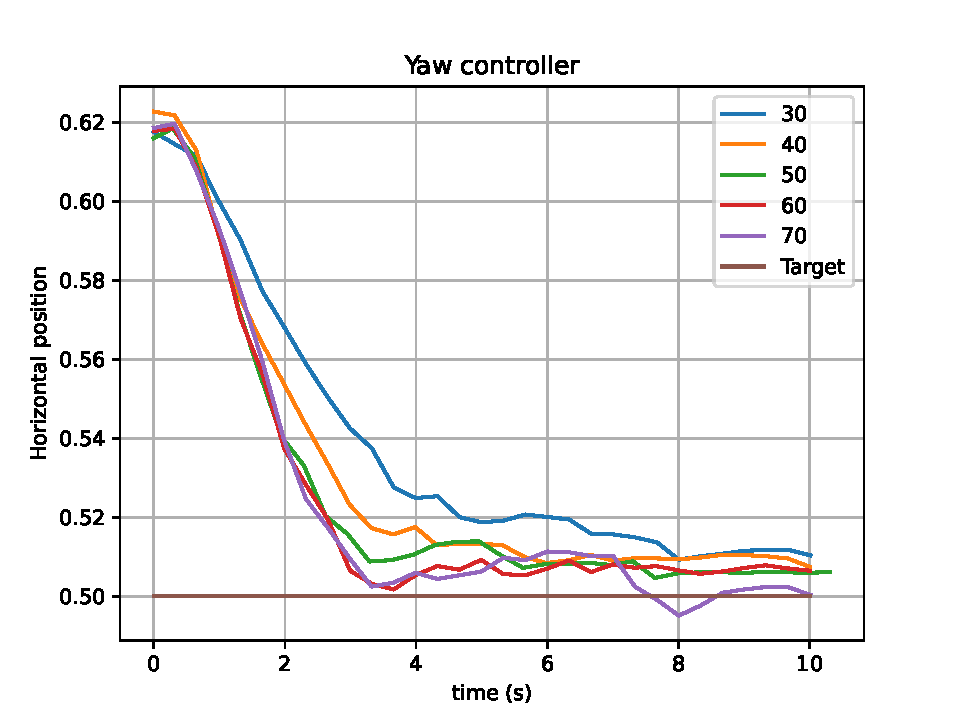
\includegraphics[width=.45\linewidth]{img/4.1-tune/yaw_p2_feedback.pdf}
  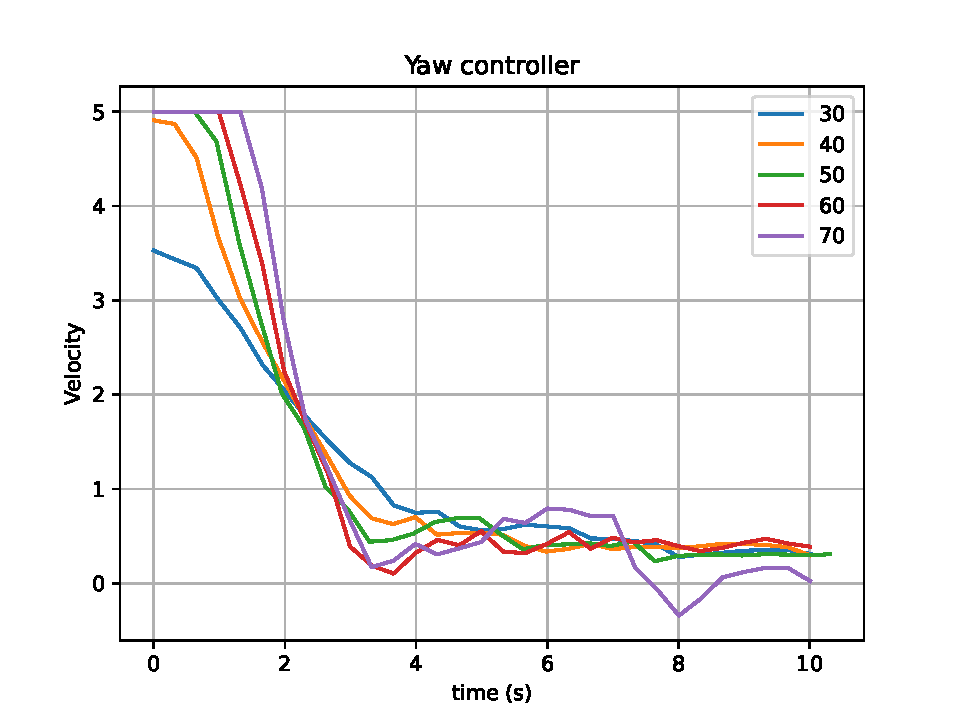
\includegraphics[width=.45\linewidth]{img/4.1-tune/yaw_p2_speed.pdf}
  \caption{Variation of (a) input position and (b) output velocity while the yaw controller is engaged for different values of $K_{P}$ between 30 and 70.}\label{fig:tune-yaw-prop2}
\end{figure}

From the values tested next in figure\ref{fig:tune-yaw-prop2}, the final value of $K_{P}=60$ is selected.
Once this approximate desired value of $K_{P}$ is decided, the derivative coefficient can be added.

\begin{figure}
  \centering
  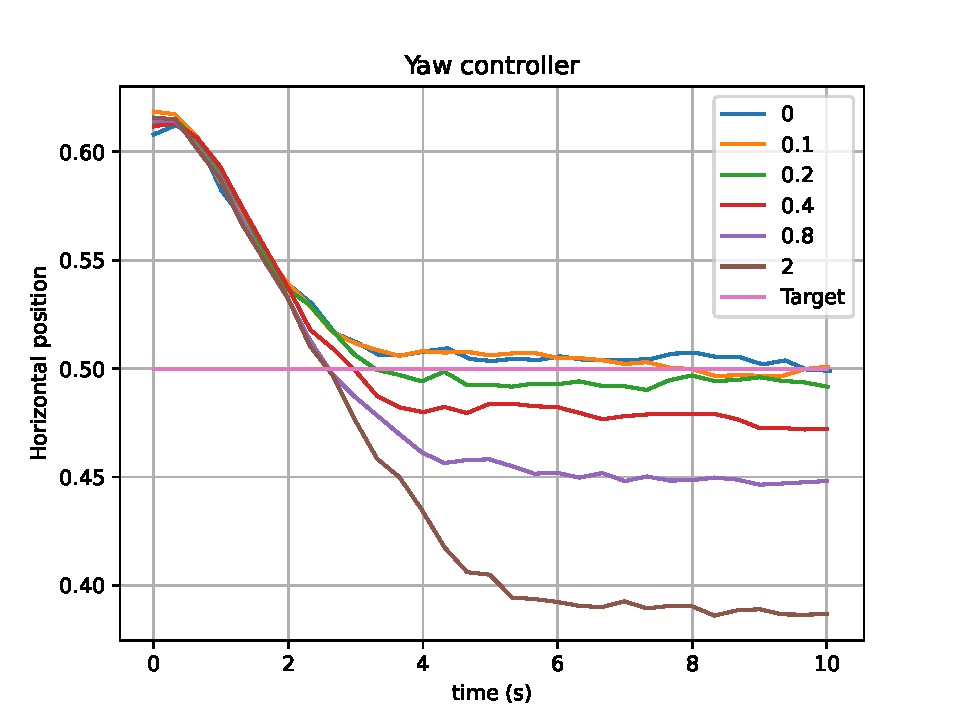
\includegraphics[width=.45\linewidth]{img/4.1-tune/yaw_i2_feedback.pdf}
  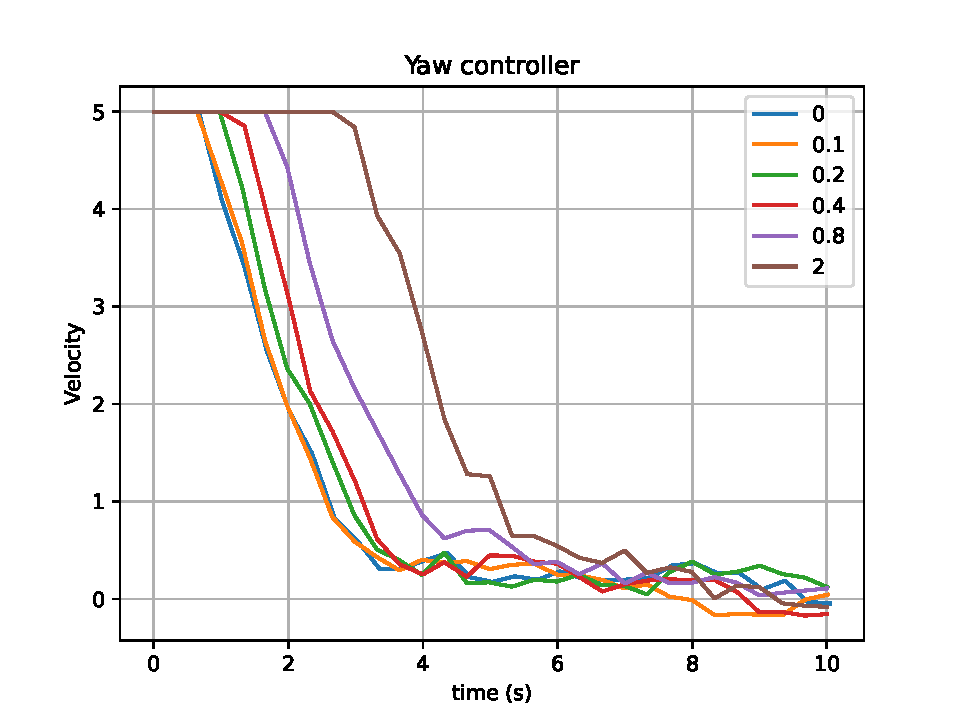
\includegraphics[width=.45\linewidth]{img/4.1-tune/yaw_i2_speed.pdf}
  \caption{Variation of (a) input position and (b) output velocity while the yaw controller is engaged for different values of $K_{I}$.}\label{fig:tune-yaw-int}
\end{figure}

\begin{figure}
  \centering
  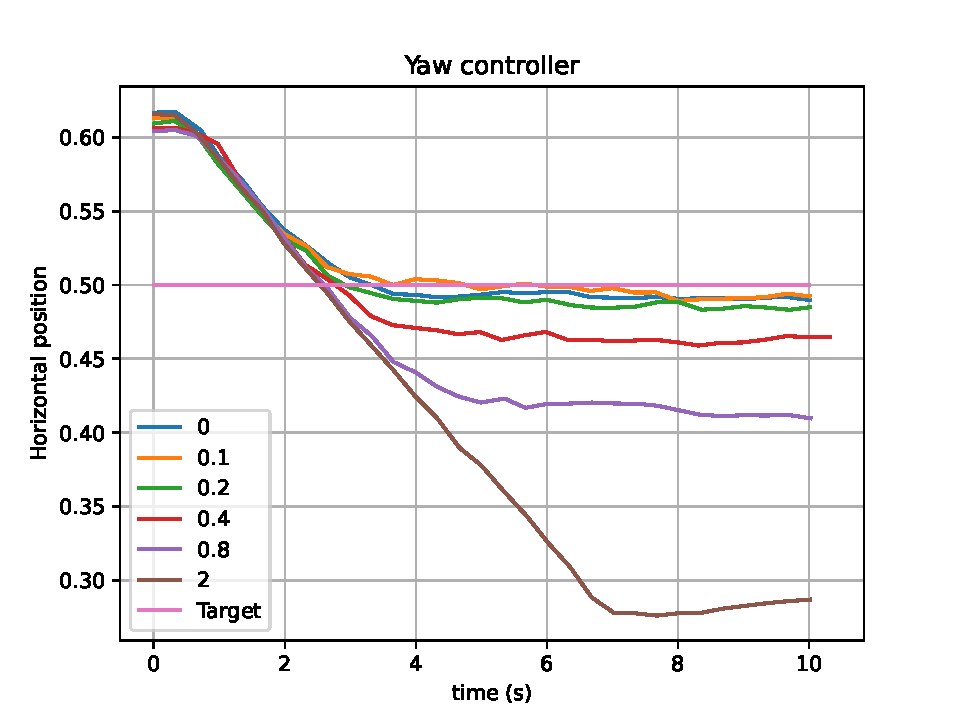
\includegraphics[width=.45\linewidth]{img/4.1-tune/yaw_d2_feedback.pdf}
  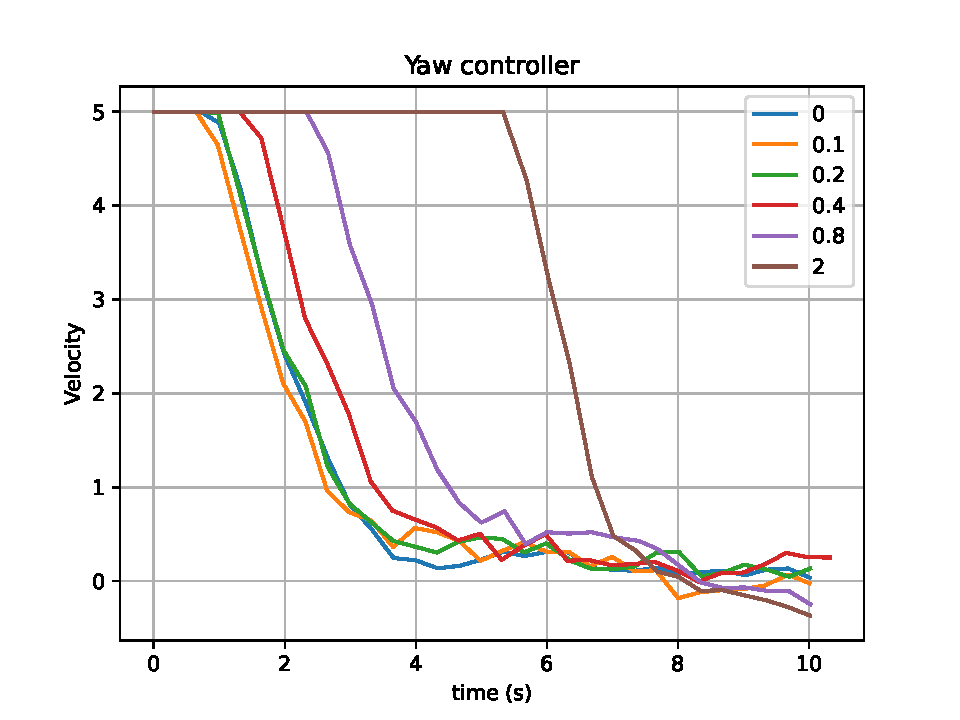
\includegraphics[width=.45\linewidth]{img/4.1-tune/yaw_d2_speed.pdf}
  \caption{Variation of (a) input position and (b) output velocity while the yaw controller is engaged for different values of $K_{D}$.}\label{fig:tune-yaw-deriv}
\end{figure}

\subsection{Forward controller}

\begin{figure}
  \centering
  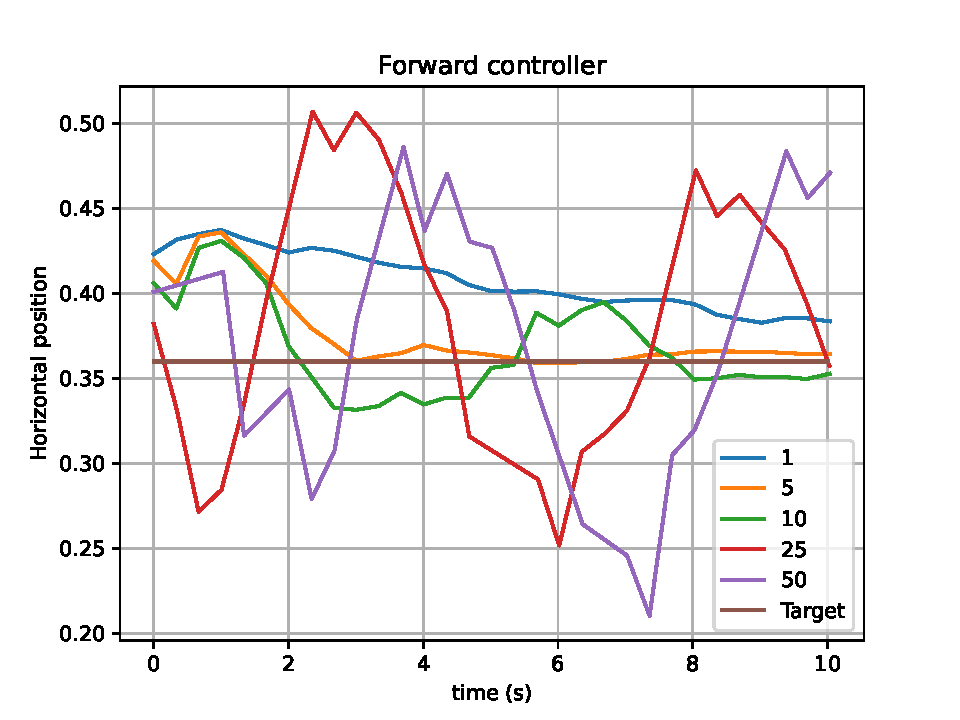
\includegraphics[width=.45\linewidth]{img/4.1-tune/fwd_p1_feedback.pdf}
  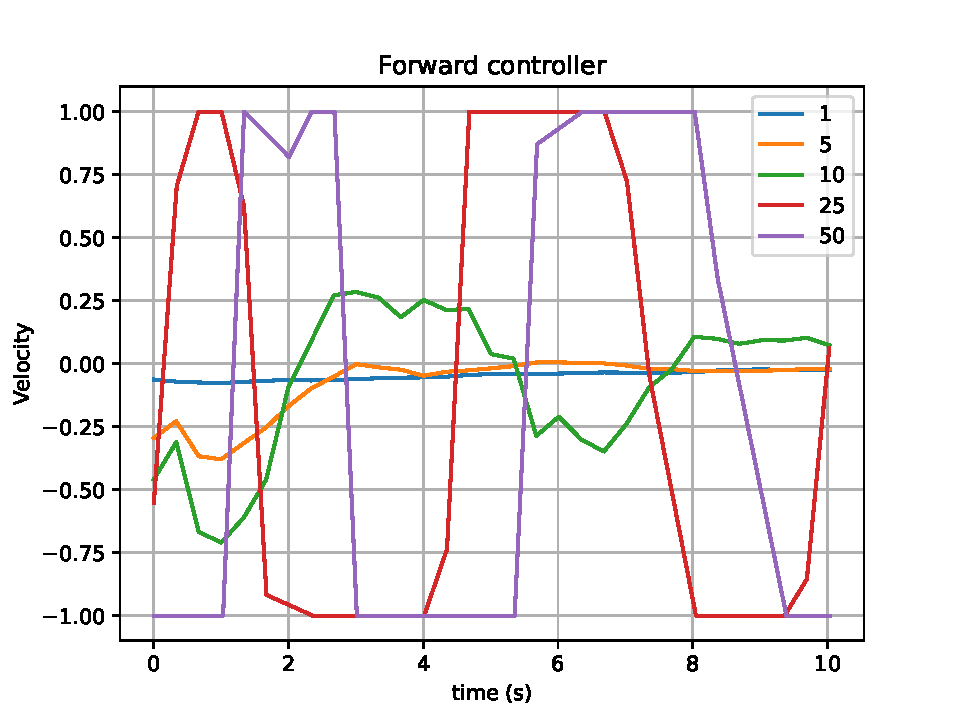
\includegraphics[width=.45\linewidth]{img/4.1-tune/fwd_p1_speed.pdf}
  \caption{Variation of (a) input position and (b) output velocity while the yaw controller is engaged for different values of $K_{D}$.}\label{fig:tune-yaw-deriv}
\end{figure}

\begin{figure}
  \centering
  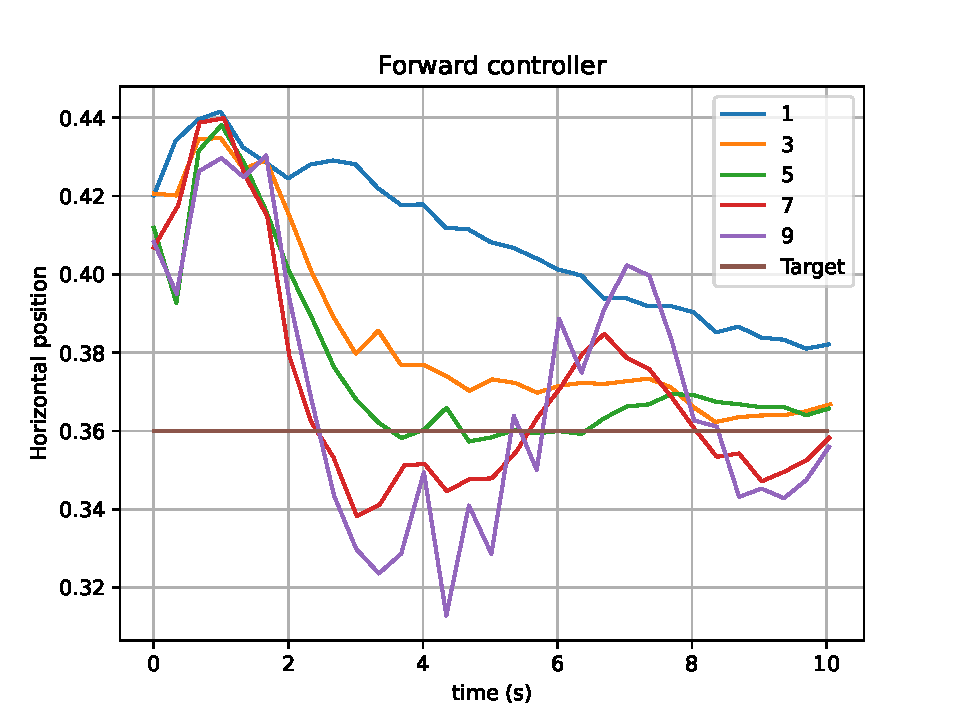
\includegraphics[width=.45\linewidth]{img/4.1-tune/fwd_p2_feedback.pdf}
  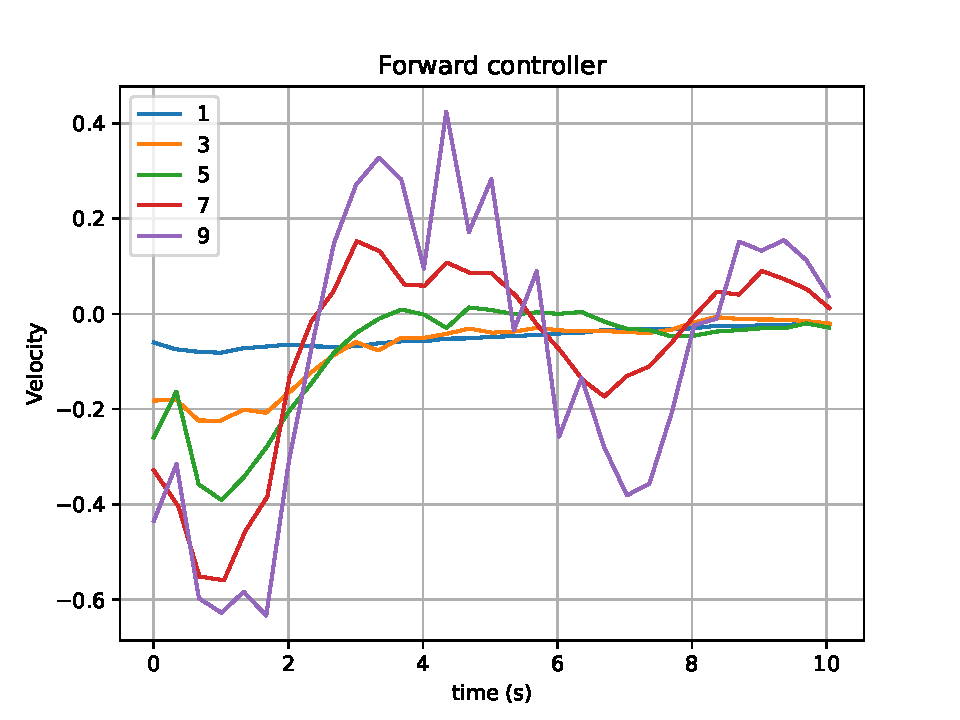
\includegraphics[width=.45\linewidth]{img/4.1-tune/fwd_p2_speed.pdf}
  \caption{Variation of (a) input position and (b) output velocity while the yaw controller is engaged for different values of $K_{D}$.}\label{fig:tune-yaw-deriv}
\end{figure}

\begin{figure}
  \centering
  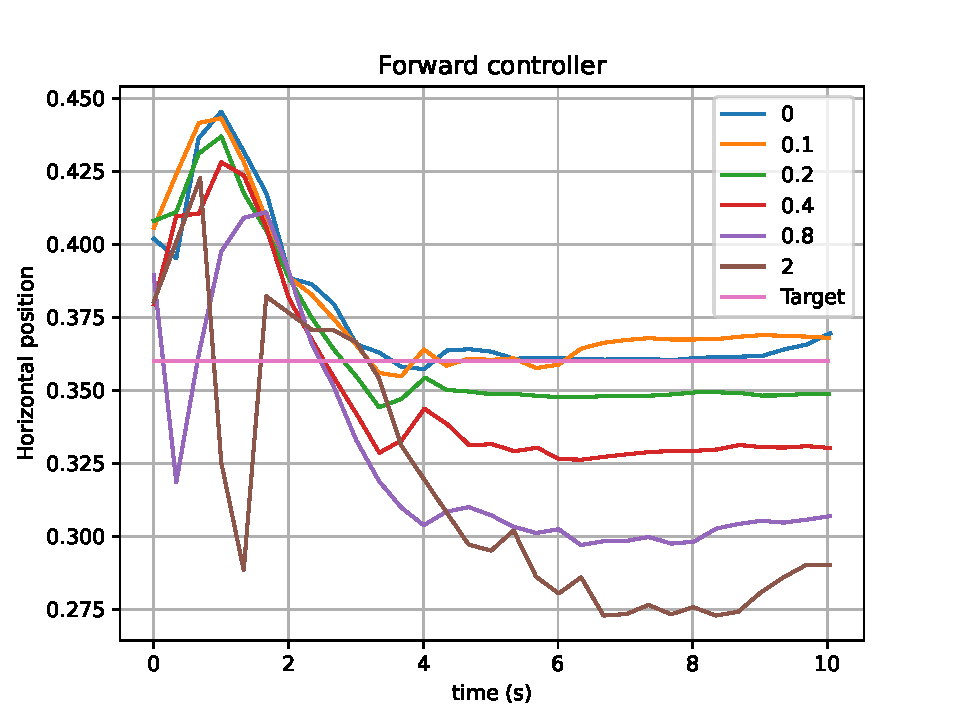
\includegraphics[width=.45\linewidth]{img/4.1-tune/fwd_i1_feedback.pdf}
  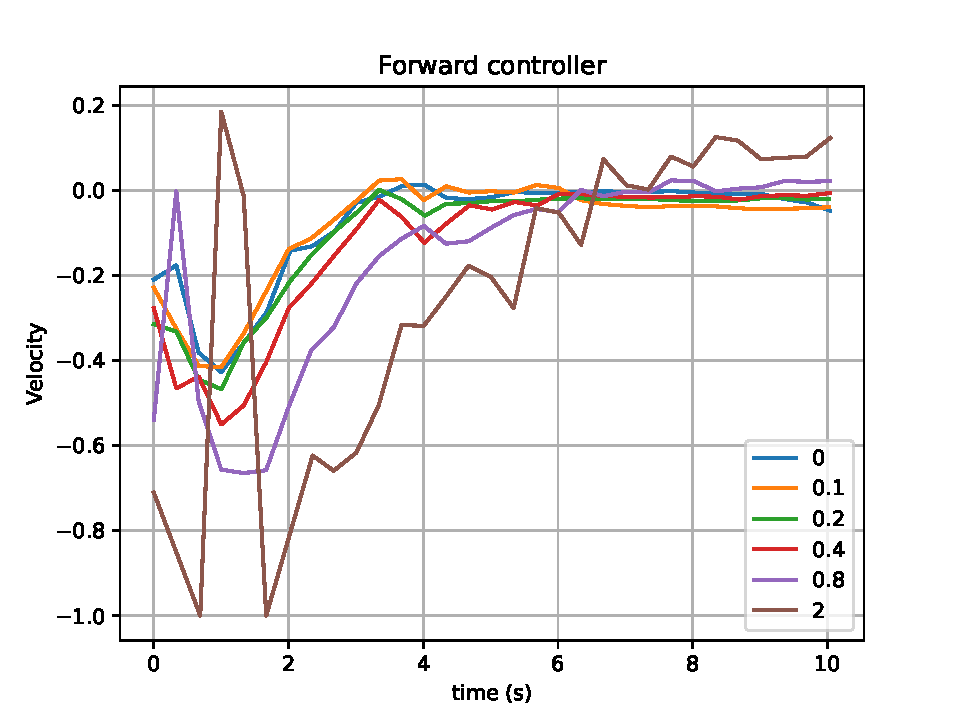
\includegraphics[width=.45\linewidth]{img/4.1-tune/fwd_i1_speed.pdf}
  \caption{Variation of (a) input position and (b) output velocity while the yaw controller is engaged for different values of $K_{D}$.}\label{fig:tune-yaw-deriv}
\end{figure}

\begin{figure}
  \centering
  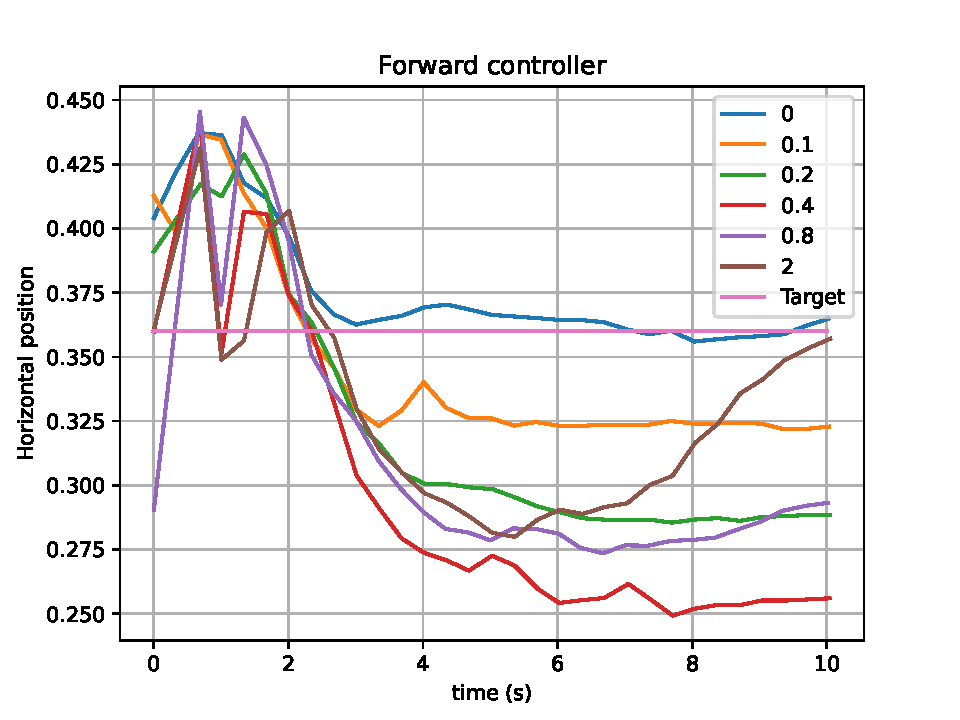
\includegraphics[width=.45\linewidth]{img/4.1-tune/fwd_d1_feedback.pdf}
  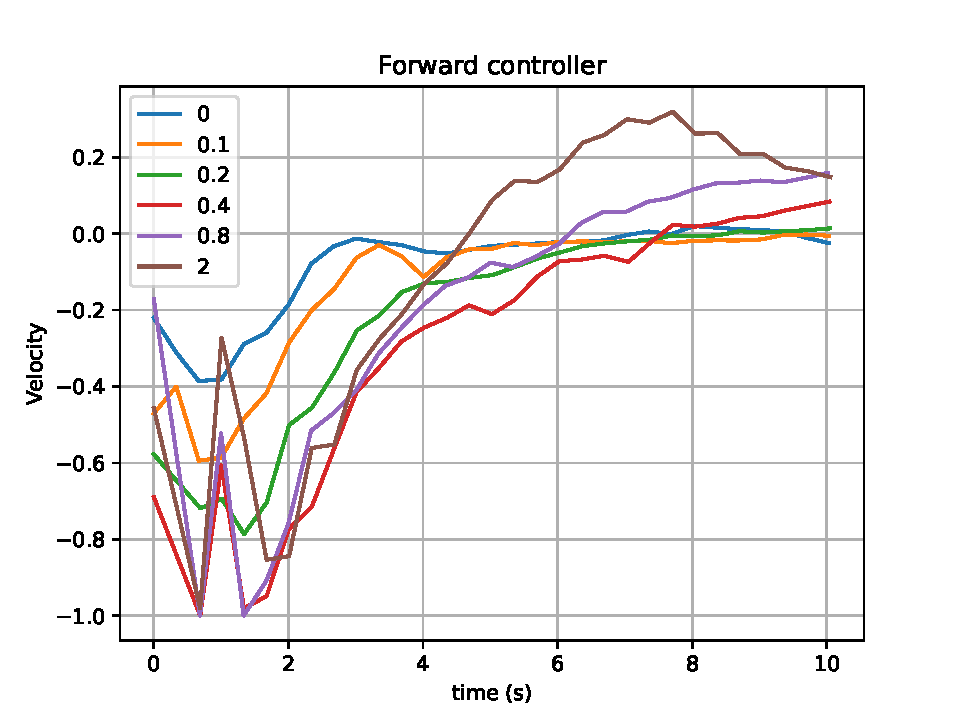
\includegraphics[width=.45\linewidth]{img/4.1-tune/fwd_d1_speed.pdf}
  \caption{Variation of (a) input position and (b) output velocity while the yaw controller is engaged for different values of $K_{D}$.}\label{fig:tune-yaw-deriv}
\end{figure}

\subsection{PID tuning validation}

\begin{figure}
  \centering
  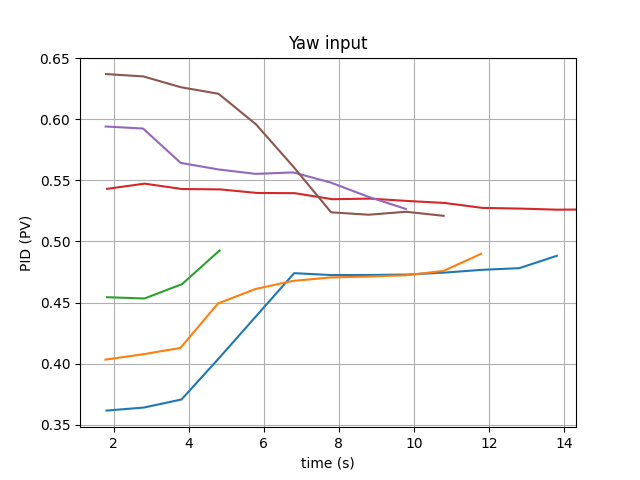
\includegraphics[width=.8\textwidth, keepaspectratio]{img/4.1-tune/yaw_validate_1.png}
  \caption{Perspective from the vehicle at the start of the program run}\label{fig:sim_camera_tune}
\end{figure}

\begin{figure}
  \centering
  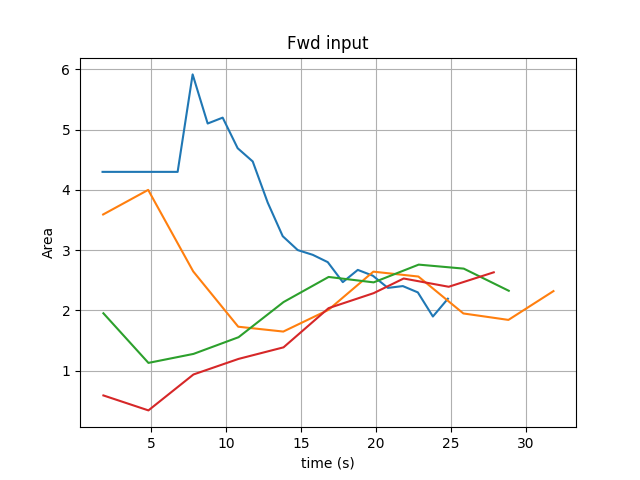
\includegraphics[width=.8\textwidth, keepaspectratio]{img/4.1-tune/fwd_validate_1.png}
  \caption{Perspective from the vehicle at the start of the program run}\label{fig:sim_camera_tune}
\end{figure}


\section{PX4 SITL simulation and validation}
\label{sec:test-2-sitl}

% Setup:    build from source code on WSL
% Test:     - Jmavsim simulator
%           - Hand solution: (on Python Windows?????)
%               - Mediapipe
%               - Pilot module
%               - Video input
% Results:  images from jmavsim, dronecontrol output, px4 console

\section{PX4 validation with AirSim}
\label{sec:test-3-airsim}

% Setup:    installing AirSim, AirSim config explanation
% Test:     - AirSim simulator
%           - Follow solution:
%               - Pose detection
%               - Images from simulator
%               - Control from PIDs
%               - Failsafes
% Results:  images from airsim, dronecontrol output, px4 console

\section{PX4 HITL simulation and validation}
\label{sec:test-4-hitl}

% Setup:    build drone, HITL configuration
% Test:     - AirSim + follow on Windows + Pixhawk
%           - QGroundControl (without program running)
%           - PX4 to computer connection
%           - RC on AirSim
% Results:  images of wiring computer-Pixhawk

\section{PX4 HITL validation with Raspberry Pi}
\label{sec:test-5-rpi}

% Setup:    Raspberry Pi installation, RPi-Pixhawk connection
% Test:     - AirSim + follow on RPi + Pixhawk
%           - Serial connection
% Results:  wiring, performance metrics

\section{PX4 HITL validation with onboard camera}
\label{sec:test-6-onboardcam}

% Setup:    installing AirSim, AirSim config explanation
% Test:     - AirSim + hand-solution on RPi + Pixhawk + onboard camera
%           - Camera holder
% Results:  holder 3d, drone close-up, camera feed

\section{Quadcopter flight tests}

\subsection{Build process}
\label{sec:test-7-builddrone}

% Setup:    build drone, configuration, calibration
% Test:     - RC, GPS, Pixhawk power supply, RPi power supply
%           - Arm, takeoff commands
% Results:  wiring, drone pictures, QGroundControl calibration screens

\subsection{Basic tests}
\label{sec:test-8-flight}

% Setup:    flight plan
% Test:     - takeoff with QGC, fly with RC
%           - tools/test_camera + record video
% Results:  video of flying

\subsection{Hand gesture control}
\label{sec:test-9-hand}

% Setup:    ...
% Test:     - Hand solution on windows through telemetry radio
%           - Free movement with offboard api
% Results:  video of flying, output from program

\subsection{Target detecting, tracking and following}
\label{sec:test-10-follow}

% Setup:    ...
% Test:     - Follow solution on RPi
%           - Controller response to real input
% Results:  video of flying, output from program
            

\cleardoublepage